\documentclass[letterpaper,twocolumn,10pt]{article}
\usepackage{epsfig,endnotes}
\begin{document}

% Don't output date
\date{}

% Title
\title{\Large
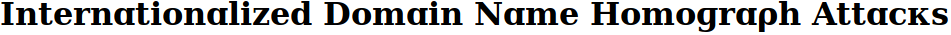
\includegraphics[height=\baselineskip]{title}
\\ \vspace{0.025 in} \large \normalfont
CSE 227: Computer Security - Spring 2017 \\ \textit{
University of California San Diego
}}

% Authors
\author{
{\rm Chen Lai}\\
\normalfont{\texttt{chl588@ucsd.edu}}
\and
{\rm Zhongrong Jian}\\
\normalfont{\texttt{zhjian@ucsd.edu}}
\and
{\rm J. Sidrach}\\
\normalfont{\texttt{jsidrach@ucsd.edu}}
}

\maketitle

\abstract{TODO}

\section{Introduction}
TODO
- Introduction to the problem
- Enumeration of sections this paper talks about

\section{Background}
TODO
- DNS: explanation
- IDN: history, explanation
- Browsers: display of IDNs, algorithms

\section{Related Work}
TODO
- Brief analysis of previous papers on the same topic

\section{Methodology}
TODO
- Introduction to the methodology
  - Reference github repository
- Subsection: data collection
  - Reference sources of data
- Subsection: data pre-processing
- Subsection: clustering, confusables algorithm
  - Caveats: not mathing /, .com, etc.
- Subsection: manual classification, guidelines used

\section{Results}
TODO
- Comment different results obtained
- Explain consequences of caveats (low number of matches)
- Explain tables
- Some other interesting results (topic-related domain hoarding)

\begin{table}[]
\centering
\begin{tabular}{|l|r|r|}
\hline
\bfseries\sffamily{Domains}                   & \bfseries\sffamily{\#}     & \bfseries\sffamily{\%}     \\ \hline
\itshape\sffamily{Canonical domain names}     & \itshape\sffamily{458731}  & \itshape\sffamily{8.31\%}  \\ \hline
\hspace{0.5cm} With IDN homographs            & 825                        & 6.04\%                     \\ \hline
\hspace{0.5cm} Without IDN homograpphs        & 457906                     & 2.27\%                     \\ \hline
\itshape\sffamily{International Domain Names} & \itshape\sffamily{1045400} & \itshape\sffamily{91.69\%} \\ \hline
\hspace{0.5cm} With canonical homograph       & 1099                       & 3.68\%                     \\ \hline
\hspace{0.5cm} Without canonical homograph    & 1044301                    & 2.74\%                     \\ \hline
\end{tabular}
\caption{Overview of the clustering results.}
\label{clustering-results}
\end{table}

\begin{table}[]
\centering
\begin{tabular}{|l|r|}
\hline
\bfseries\sffamily{Domain} & \bfseries\sffamily{\# of IDN homographs} \\ \hline
google.com                 & 24                                       \\ \hline
youtube.com                & 3                                        \\ \hline
facebook.com               & 9                                        \\ \hline
baidu.com                  & 3                                        \\ \hline
yahoo.com                  & 4                                        \\ \hline
reddit.com                 & 1                                        \\ \hline
qq.com                     & 2                                        \\ \hline
taobao.com                 & 1                                        \\ \hline
live.com                   & 1                                        \\ \hline
vk.com                     & 6                                        \\ \hline
\end{tabular}
\caption{Top ten .com domains in the Alexa ranking with IDN homographs.}
\label{top-com-alexa-with-idns}
\end{table}

\begin{table}[]
\centering
\begin{tabular}{|l|r|r|}
\hline
\bfseries\sffamily{Status}           & \bfseries\sffamily{\#} & \bfseries\sffamily{\%}     \\ \hline
\itshape\sffamily{Canonical}         & \itshape\sffamily{88}  & \itshape\sffamily{8.31\%}  \\ \hline
\hspace{0.5cm} Parking               & 64                     & 6.04\%                     \\ \hline
\hspace{0.5cm} Redirect              & 24                     & 2.27\%                     \\ \hline
\itshape\sffamily{Third Party}       & \itshape\sffamily{971} & \itshape\sffamily{91.69\%} \\ \hline
\hspace{0.5cm} Redirect to Canonical & 39                     & 3.68\%                     \\ \hline
\hspace{0.5cm} Unrelated             & 29                     & 2.74\%                     \\ \hline
\hspace{0.5cm} Parking               & 872                    & 82.34\%                    \\ \hline
\hspace{0.5cm} Scam                  & 31                     & 2.93\%                     \\ \hline
\end{tabular}
\caption{Breakdown of the manually classified homograph IDNs.}
\label{manually-classified-idns}
\end{table}

TODO: mention:
  Number of Third Party domains whose Registrant Organization and Email has than one homograph IDN registered: 437
  Number of Registrant's Organization and Email that have more than one homograph IDN: 82

\begin{table*}[]
\centering
\begin{tabular}{|l|l|r|}
\hline
\bfseries\sffamily{Registrant organization} & \bfseries\sffamily{Registrant email} & \bfseries\sffamily{\# of homograph IDNs} \\ \hline
Domains By Proxy, LLC                & --                         & 89                                                        \\ \hline
Super Privacy Service c/o Dynadot    & privacy@dynadot.com        & 23                                                        \\ \hline
Domain Registries Foundation         & --                         & 22                                                        \\ \hline
Duong Thien                          & thiendv@outlook.com        & 18                                                        \\ \hline
Syngenuity Limited                   & manager@syngenuity.com     & 12                                                        \\ \hline
Helpnet: Brand Development \& Sales  & help@strongestbrands.com   & 12                                                        \\ \hline
ONUNO L.L.C.                         & corucas@gmail.com          & 11                                                        \\ \hline
Privacy Protection Service INC d/b/a & contact@privacyprotect.org & 10                                                        \\ \hline
Hubertus Henz                        & hu\_h5@yahoo.de            & 9                                                         \\ \hline
wuyu                                 & wy65535@126.com            & 7                                                         \\ \hline
\end{tabular}
\caption{Top ten registrants with the most homograph IDNs.}
\label{top-registrants-homograph-idns}
\end{table*}

\section{Ethical Considerations}
TODO
- Brief explanation why this research is ethical

\section{Conclusions}
TODO
- Conclusions of our work
- Possible future work

TODO DELETE~\cite{ipv4sta}\endnote{Endnote}

\section*{Acknowledgements}
We would like to thank Louis DeKoven and Stefan Savage for their help and support throughout this project.

{\footnotesize \bibliographystyle{acm}
\bibliography{bibliography}}

\theendnotes

\end{document}
